\section{Results} \label{sc:results}
The algorithms were evaluated under the conditions presented in Section \ref{sc:experimental-validation}. The results of the evaluation for each algorithm are presented in the following sections.

\subsection{Parameter influence}
K-SVD algorithm, as presented in Section \ref{sc:description-ksvd}, requires to tune up some parameters. Each variable was varied during the evaluation process to observe its impact on the results. In general, the observed impact was the following:

\subsubsection{Block size}
Block size: The block size represents the dimension of the patch to consider. On one hand, when evaluating synthetic images, the higher the value of the parameter, the more blurred the result. On the other hand, the best results for SD-OCT was obtained when using a block size of 32 -- the biggest value tested for this parameter.

\begin{figure}[H]
  \centering
 \begin{tabular}{c c c c c}
     \begin{varwidth}{0.5\linewidth}
       \subfigure{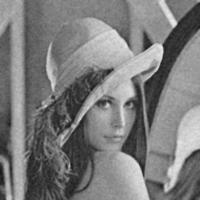
\includegraphics[width=16mm]{Figures/lena_block_size_4.jpg}}
     \end{varwidth}
     \begin{varwidth}{0.5\linewidth}
       \subfigure{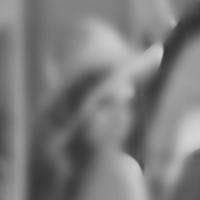
\includegraphics[width=16mm]{Figures/lena_block_size_32.jpg}}
     \end{varwidth}
 \end{tabular}
  \caption{Denoised images with K-SVD algorithm using different block sizes. On the left the block size is 4 while on the right is 32.} 
  \label{fig:influence-block-size}
\end{figure}

\subsubsection{Dictionary size}
This parameter determines the number of patches to consider for the dictionary. The size by itself does not modify the result dramatically.

\begin{figure}[H]
  \centering
 \begin{tabular}{c c c c c}
     \begin{varwidth}{0.5\linewidth}
       \subfigure{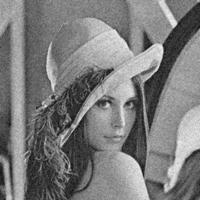
\includegraphics[width=16mm]{Figures/lena_dic_size_256.jpg}}
     \end{varwidth}
     \begin{varwidth}{0.5\linewidth}
       \subfigure{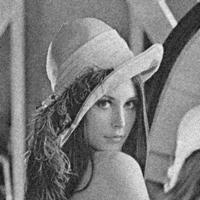
\includegraphics[width=16mm]{Figures/lena_dic_size_512.jpg}}
     \end{varwidth}
 \end{tabular}
  \caption{Denoised images with K-SVD algorithm using different dictionary sizes. On the left the dictionary size is 256 while on the right is 512.} 
  \label{fig:influence-dictionary-size}
\end{figure}

\subsubsection{Training iterations (Trainnum)}
This value corresponds to the number of iterations performed during the training step. Usually, when it increases, the result is better. However, we observed that there is a limit for which no better result is obtained. It is required that its value must be greater or equal to the dictionary size.

\subsubsection{Gain}
The influence of this parameter is seen on the edges of the resulting images. When its value is decreased, the image is less denoised but the edges were better preserved.

\subsubsection{Maximum number of atoms (maxatoms)}
This parameter is related to the number of elements on the dictionary to consider when reconstructing a patch of the noisy image. The higher the value, the better the reconstruction but also the slower the algorithm gets. Thus, the idea is to find the minimum value such that the trade-off between reconstruction and computation time is balanced. 
 
\subsubsection{Noise estimation} \label{sc:noise-estimation}
As stated previously, the level of distortion on the SD-OCT images is not known beforehand and this value is required by the K-SVD algorithm. Then, the estimation of this parameter is carried out. The method consists in taking an homogenous patch of the image and, by looking at the histogram, determine the sigma value. The observed value for sigma among the test set was around $10$. Moreover, we calculated this parameter for different retinopathy volumes getting similar results.

\subsection{Synthetic images} \label{sc:results_synthetic}
In this section, the obtained results of denoising the synthetic images with the methods explained in Section \ref{sc:state-of-the-art} are shown. 

First, the mean, median, local statistics and wavelet filters are evaluated with the synthetic images of Section \ref{sc:experimental_sythetic}. After that, the K-SVD filter is applied in such images. With these last results, proper comparisons are done between the K-SVD and the traditional denoising algorithms.

\subsubsection{Mean filter}

\begin{figure}[H]
  \centering
  \begin{tabular}{c c c c c}
      \begin{varwidth}{0.5\linewidth}
        \subfigure{\includegraphics[width=16mm]{Figures/results_mean/color_lena_nor_f.jpg}}\\
        \subfigure{\includegraphics[width=16mm]{Figures/results_mean/color_cameraman_nor_f.jpg}}\\
        \subfigure{\includegraphics[width=16mm]{Figures/results_mean/color_baboon_nor_f.jpg}}
      \end{varwidth}
      \begin{varwidth}{0.5\linewidth}
        \subfigure{\includegraphics[width=16mm]{Figures/results_mean/color_lena_ric_f.jpg}}\\
        \subfigure{\includegraphics[width=16mm]{Figures/results_mean/color_cameraman_ric_f.jpg}}\\
        \subfigure{\includegraphics[width=16mm]{Figures/results_mean/color_baboon_ric_f.jpg}}
      \end{varwidth}
      \begin{varwidth}{0.5\linewidth}
        \subfigure{\includegraphics[width=16mm]{Figures/results_mean/color_lena_uni_f.jpg}}\\
        \subfigure{\includegraphics[width=16mm]{Figures/results_mean/color_cameraman_uni_f.jpg}}\\
        \subfigure{\includegraphics[width=16mm]{Figures/results_mean/color_baboon_uni_f.jpg}}
      \end{varwidth}
      \begin{varwidth}{0.5\linewidth}
        \subfigure{\includegraphics[width=16mm]{Figures/results_mean/color_lena_sp_f.jpg}}\\
        \subfigure{\includegraphics[width=16mm]{Figures/results_mean/color_cameraman_sp_f.jpg}}\\
        \subfigure{\includegraphics[width=16mm]{Figures/results_mean/color_baboon_sp_f.jpg}}
      \end{varwidth}
      \begin{varwidth}{0.5\linewidth}
        \subfigure{\includegraphics[width=16mm]{Figures/results_mean/color_lena_spec.jpg}}\\
        \subfigure{\includegraphics[width=16mm]{Figures/results_mean/color_cameraman_spec.jpg}}\\
        \subfigure{\includegraphics[width=16mm]{Figures/results_mean/color_baboon_spec.jpg}}
      \end{varwidth}
  	\end{tabular}
  \caption{Denoised images with the mean filter represented in a colormap format. From left to right: additive Gaussian, additive Rician, additive uniform, additive salt and pepper and multiplicative speckle noise, respectively.} 
  \label{fig:results_mean_c}
\end{figure}

\subsubsection{Median filter}

\begin{figure}[H]
  \centering
  \begin{tabular}{c c c c c}
      \begin{varwidth}{0.5\linewidth}
        \subfigure{\includegraphics[width=16mm]{Figures/results_median/color_lena_nor_f.jpg}}\\
        \subfigure{\includegraphics[width=16mm]{Figures/results_median/color_cameraman_nor_f.jpg}}\\
        \subfigure{\includegraphics[width=16mm]{Figures/results_median/color_baboon_nor_f.jpg}}
      \end{varwidth}
      \begin{varwidth}{0.5\linewidth}
        \subfigure{\includegraphics[width=16mm]{Figures/results_median/color_lena_ric_f.jpg}}\\
        \subfigure{\includegraphics[width=16mm]{Figures/results_median/color_cameraman_ric_f.jpg}}\\
        \subfigure{\includegraphics[width=16mm]{Figures/results_median/color_baboon_ric_f.jpg}}
      \end{varwidth}
      \begin{varwidth}{0.5\linewidth}
        \subfigure{\includegraphics[width=16mm]{Figures/results_median/color_lena_uni_f.jpg}}\\
        \subfigure{\includegraphics[width=16mm]{Figures/results_median/color_cameraman_uni_f.jpg}}\\
        \subfigure{\includegraphics[width=16mm]{Figures/results_median/color_baboon_uni_f.jpg}}
      \end{varwidth}
      \begin{varwidth}{0.5\linewidth}
        \subfigure{\includegraphics[width=16mm]{Figures/results_median/color_lena_sp_f.jpg}}\\
        \subfigure{\includegraphics[width=16mm]{Figures/results_median/color_cameraman_sp_f.jpg}}\\
        \subfigure{\includegraphics[width=16mm]{Figures/results_median/color_baboon_sp_f.jpg}}
      \end{varwidth}
\begin{varwidth}{0.5\linewidth}
        \subfigure{\includegraphics[width=16mm]{Figures/results_median/color_lena_spec.jpg}}\\
        \subfigure{\includegraphics[width=16mm]{Figures/results_median/color_cameraman_spec.jpg}}\\
        \subfigure{\includegraphics[width=16mm]{Figures/results_median/color_baboon_spec.jpg}}
      \end{varwidth}
  	\end{tabular}
  \caption{Denoised images with the median filter represented in a colormap format. From left to right: additive Gaussian, additive Rician, additive uniform, additive salt and pepper and multiplicative speckle noise, respectively.} 
  \label{fig:Figures/results_Lee_c}
\end{figure}


\subsubsection{LS filter}

\begin{figure}[H]
  \centering
  \begin{tabular}{c c c c c}
      \begin{varwidth}{0.5\linewidth}
        \subfigure{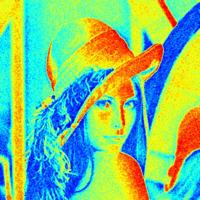
\includegraphics[width=16mm]{Figures/results_Lee/color_lena_nor-denoised.jpg}}\\
        \subfigure{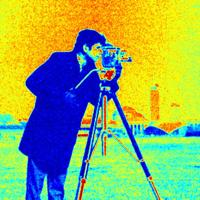
\includegraphics[width=16mm]{Figures/results_Lee/color_cameraman_nor-denoised.jpg}}\\
        \subfigure{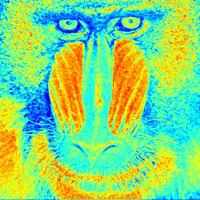
\includegraphics[width=16mm]{Figures/results_Lee/color_baboon_nor-denoised.jpg}}
      \end{varwidth}
      \begin{varwidth}{0.5\linewidth}
        \subfigure{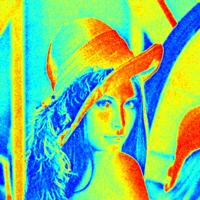
\includegraphics[width=16mm]{Figures/results_Lee/color_lena_ric-denoised.jpg}}\\
        \subfigure{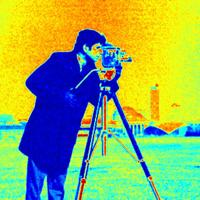
\includegraphics[width=16mm]{Figures/results_Lee/color_cameraman_ric-denoised.jpg}}\\
        \subfigure{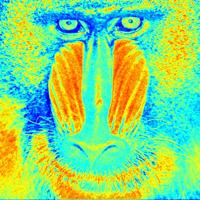
\includegraphics[width=16mm]{Figures/results_Lee/color_baboon_ric-denoised.jpg}}
      \end{varwidth}
      \begin{varwidth}{0.5\linewidth}
        \subfigure{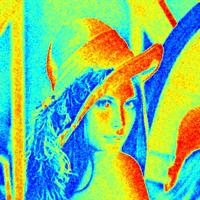
\includegraphics[width=16mm]{Figures/results_Lee/color_lena_uni-denoised.jpg}}\\
        \subfigure{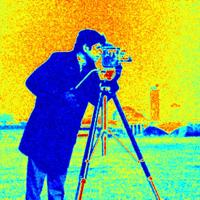
\includegraphics[width=16mm]{Figures/results_Lee/color_cameraman_uni-denoised.jpg}}\\
        \subfigure{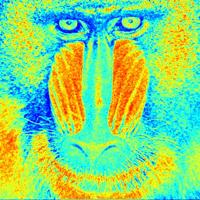
\includegraphics[width=16mm]{Figures/results_Lee/color_baboon_uni-denoised.jpg}}
      \end{varwidth}
      \begin{varwidth}{0.5\linewidth}
        \subfigure{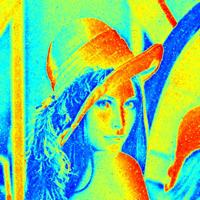
\includegraphics[width=16mm]{Figures/results_Lee/color_lena_sp-denoised.jpg}}\\
        \subfigure{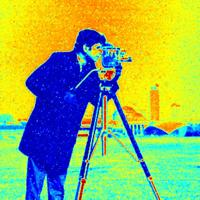
\includegraphics[width=16mm]{Figures/results_Lee/color_cameraman_sp-denoised.jpg}}\\
        \subfigure{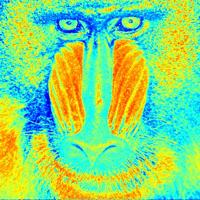
\includegraphics[width=16mm]{Figures/results_Lee/color_baboon_sp-denoised.jpg}}
      \end{varwidth}
      \begin{varwidth}{0.5\linewidth}
        \subfigure{\includegraphics[width=16mm]{Figures/results_Lee/color_lena_spec.jpg}}\\
        \subfigure{\includegraphics[width=16mm]{Figures/results_Lee/color_cameraman_spec.jpg}}\\
        \subfigure{\includegraphics[width=16mm]{Figures/results_Lee/color_baboon_spec.jpg}}
      \end{varwidth}
  	\end{tabular}
  \caption{Denoised images with the LS filter represented in a colormap format. From left to right: additive Gaussian, additive Rician, additive uniform, additive salt and pepper and multiplicative speckle noise, respectively.} 
  \label{fig:results_lee}
\end{figure}

\subsubsection{Wavelet filter}

\begin{figure}[H]
  \centering
  \begin{tabular}{c c c c c}
      \begin{varwidth}{0.5\linewidth}
        \subfigure{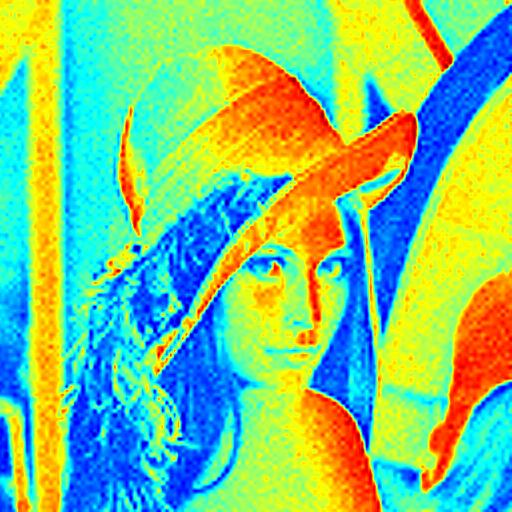
\includegraphics[width=16mm]{Figures/results_wavelet/color_lena_nor.jpg}}\\
        \subfigure{\includegraphics[width=16mm]{Figures/results_wavelet/color_cameraman_nor.jpg}}\\
        \subfigure{\includegraphics[width=16mm]{Figures/results_wavelet/color_baboon_nor.jpg}}
      \end{varwidth}
      \begin{varwidth}{0.5\linewidth}
        \subfigure{\includegraphics[width=16mm]{Figures/results_wavelet/color_lena_ric.jpg}}\\
        \subfigure{\includegraphics[width=16mm]{Figures/results_wavelet/color_cameraman_ric.jpg}}\\
        \subfigure{\includegraphics[width=16mm]{Figures/results_wavelet/color_baboon_ric.jpg}}
      \end{varwidth}
      \begin{varwidth}{0.5\linewidth}
        \subfigure{\includegraphics[width=16mm]{Figures/results_wavelet/color_lena_uni.jpg}}\\
        \subfigure{\includegraphics[width=16mm]{Figures/results_wavelet/color_cameraman_uni.jpg}}\\
        \subfigure{\includegraphics[width=16mm]{Figures/results_wavelet/color_baboon_uni.jpg}}
      \end{varwidth}
      \begin{varwidth}{0.5\linewidth}
        \subfigure{\includegraphics[width=16mm]{Figures/results_wavelet/color_lena_sp.jpg}}\\
        \subfigure{\includegraphics[width=16mm]{Figures/results_wavelet/color_cameraman_sp.jpg}}\\
        \subfigure{\includegraphics[width=16mm]{Figures/results_wavelet/color_baboon_sp.jpg}}
      \end{varwidth}
      \begin{varwidth}{0.5\linewidth}
        \subfigure{\includegraphics[width=16mm]{Figures/results_wavelet/color_lena_spec.jpg}}\\
        \subfigure{\includegraphics[width=16mm]{Figures/results_wavelet/color_cameraman_spec.jpg}}\\
        \subfigure{\includegraphics[width=16mm]{Figures/results_wavelet/color_baboon_spec.jpg}}
      \end{varwidth}
  	\end{tabular}
  \caption{Denoised images with the wavelet filter represented in a colormap format. From left to right: additive Gaussian, additive Rician, additive uniform, additive salt and pepper and multiplicative speckle noise, respectively.} 
  \label{fig:results_wavelet_c}
\end{figure}

\subsubsection{K-SVD filter}
%The obtained results for the K-SVD filter are shown in Fig. \ref{fig:results_synthetic_ksvd}.

\begin{figure}[H]
  \centering
  \begin{tabular}{c c c c c}
      \begin{varwidth}{0.5\linewidth}
        \subfigure{\includegraphics[width=16mm]{Figures/results_KSVD/color_lena_nor.jpg}}\\
        \subfigure{\includegraphics[width=16mm]{Figures/results_KSVD/color_cameraman_nor.jpg}}\\
        \subfigure{\includegraphics[width=16mm]{Figures/results_KSVD/color_baboon_nor.jpg}}
      \end{varwidth}
      \begin{varwidth}{0.5\linewidth}
        \subfigure{\includegraphics[width=16mm]{Figures/results_KSVD/color_lena_ric.jpg}}\\
        \subfigure{\includegraphics[width=16mm]{Figures/results_KSVD/color_cameraman_ric.jpg}}\\
        \subfigure{\includegraphics[width=16mm]{Figures/results_KSVD/color_baboon_ric.jpg}}
      \end{varwidth}
      \begin{varwidth}{0.5\linewidth}
        \subfigure{\includegraphics[width=16mm]{Figures/results_KSVD/color_lena_uni.jpg}}\\
        \subfigure{\includegraphics[width=16mm]{Figures/results_KSVD/color_cameraman_uni.jpg}}\\
        \subfigure{\includegraphics[width=16mm]{Figures/results_KSVD/color_baboon_uni.jpg}}
      \end{varwidth}
      \begin{varwidth}{0.5\linewidth}
        \subfigure{\includegraphics[width=16mm]{Figures/results_KSVD/color_lena_sp.jpg}}\\
        \subfigure{\includegraphics[width=16mm]{Figures/results_KSVD/color_cameraman_sp.jpg}}\\
        \subfigure{\includegraphics[width=16mm]{Figures/results_KSVD/color_baboon_sp.jpg}}
      \end{varwidth}
      \begin{varwidth}{0.5\linewidth}
        \subfigure{\includegraphics[width=16mm]{Figures/results_KSVD/color_lena_spec.jpg}}\\
        \subfigure{\includegraphics[width=16mm]{Figures/results_KSVD/color_cameraman_spec.jpg}}\\
        \subfigure{\includegraphics[width=16mm]{Figures/results_KSVD/color_baboon_spec.jpg}}
      \end{varwidth}
  	\end{tabular}
  \caption{Denoised images with the K-SVD filter. From left to right: removing Gaussian, Rician, uniform, salt and pepper and speckle noise, respectively.} 
  \label{fig:results_synthetic_ksvd}
\end{figure}

The comparative results are shown in Fig. \ref{fig:results_synthetic_ksvd_evaluation}. It can be seen that the PSNR of the initial noise is improved in most of the cases except for Baboon test set in which the results are the same or worse. In general, Baboon is the test set leading to the worst restoration for all the evaluated algorithms. This fact could be a consequence of the characteristics of the spiky hair of the baboon. These spikes form a set of edges which can be ``easily'' affected by adding noise and also by restoring with the considered algorithms. Thus, when the denoising process is carried out on this section, most of it, which is formed by high frequencies, is lost.

\begin{figure}[H]
  \centering
     \subfigure{\includegraphics[width=80mm]{Figures/results_KSVD/_comparison.jpg}}
  \caption{Comparison of the K-SVD filter with traditional filtering techniques.} 
  \label{fig:results_synthetic_ksvd_evaluation}
\end{figure}

K-SVD algorithm is able to remove noise from the different test images. However, its performance was not always the best. It can be observed that in some cases, the values of PSNR for mean filter and median filter are higher than the ones for K-SVD. Contrarily, we see that the wavelet filter does not succeed in filtering any of the types of noise, compared to other methods. 

As expected, median filter outperforms when evaluated under salt and pepper noise in comparison with the other algorithms. 


\subsection{Retinopathy images} 
To provide a quantitative comparison of the denoised retinopathy images with the different methods, we computed the PSNR. In this case, it was performed between the input image and the output of each algorithm. It is clear that although this computation does not give the real PSNR, the obtained value is useful to get an idea of the performance of the different algorithms. In general terms, K-SVD is able to reduce noise on the image without affecting the key components (the layers on the images) more than the other algorithms.

\begin{figure}[H]
  \centering
      \subfigure{\includegraphics[width=80mm]{Figures/results_KSVD/retinopathy_image.jpg}}
  \caption{Denoised retinopathy image with the K-SVD filter.} 
  \label{fig:results_rimage_ksvd}
\end{figure}

\begin{figure}[H]
  \centering
      \subfigure{\includegraphics[width=80mm]{Figures/results_KSVD/retinopathy_segmentation.jpg}}
  \caption{Segmentation of a retinopathy volume after denoising using the K-SVD filter.} 
  \label{fig:results_rsegmentation_ksvd}
\end{figure}
